\documentclass[a4paper, 10pt]{article}
\usepackage[english]{babel}
\usepackage[utf8]{inputenc}
\usepackage{enumitem}
\usepackage{titlesec}
\usepackage{framed}
\usepackage{listings}
\usepackage{graphicx}
\usepackage{titling}
\usepackage{blindtext}
\usepackage{amsmath}  % for \hookrightarrow
\usepackage{xcolor}   % for \textcolor
\graphicspath{ {./ER/} }
\usepackage[hmargin=2cm,vmargin=3.5cm,bmargin=2cm]{geometry}

\setlist[itemize]{noitemsep, topsep=0pt}
\setlength\parindent{0pt}

\setcounter{secnumdepth}{0} %% no numbering

\begin{document}
\title{Advanced DataBases, First Delivery\\
  \huge Bank Management System}
\author{
  Samuel Lúcio Vicente, 251720
  \and
  Daniel Silva, 251702
  \and
  Jorge Espanhol, XXXXXX
}

\date{Politechnika Wrocławska\\C4 Group\\\today}

\maketitle

\lstset{
  basicstyle=\small\ttfamily,
  frame=lrtb,
  numbers=left,
  columns=fullflexible,
  breaklines=true,
  postbreak=\mbox{\textcolor{red}{$\hookrightarrow$}\space}
}

\section{Short Description}


\section{ERD}
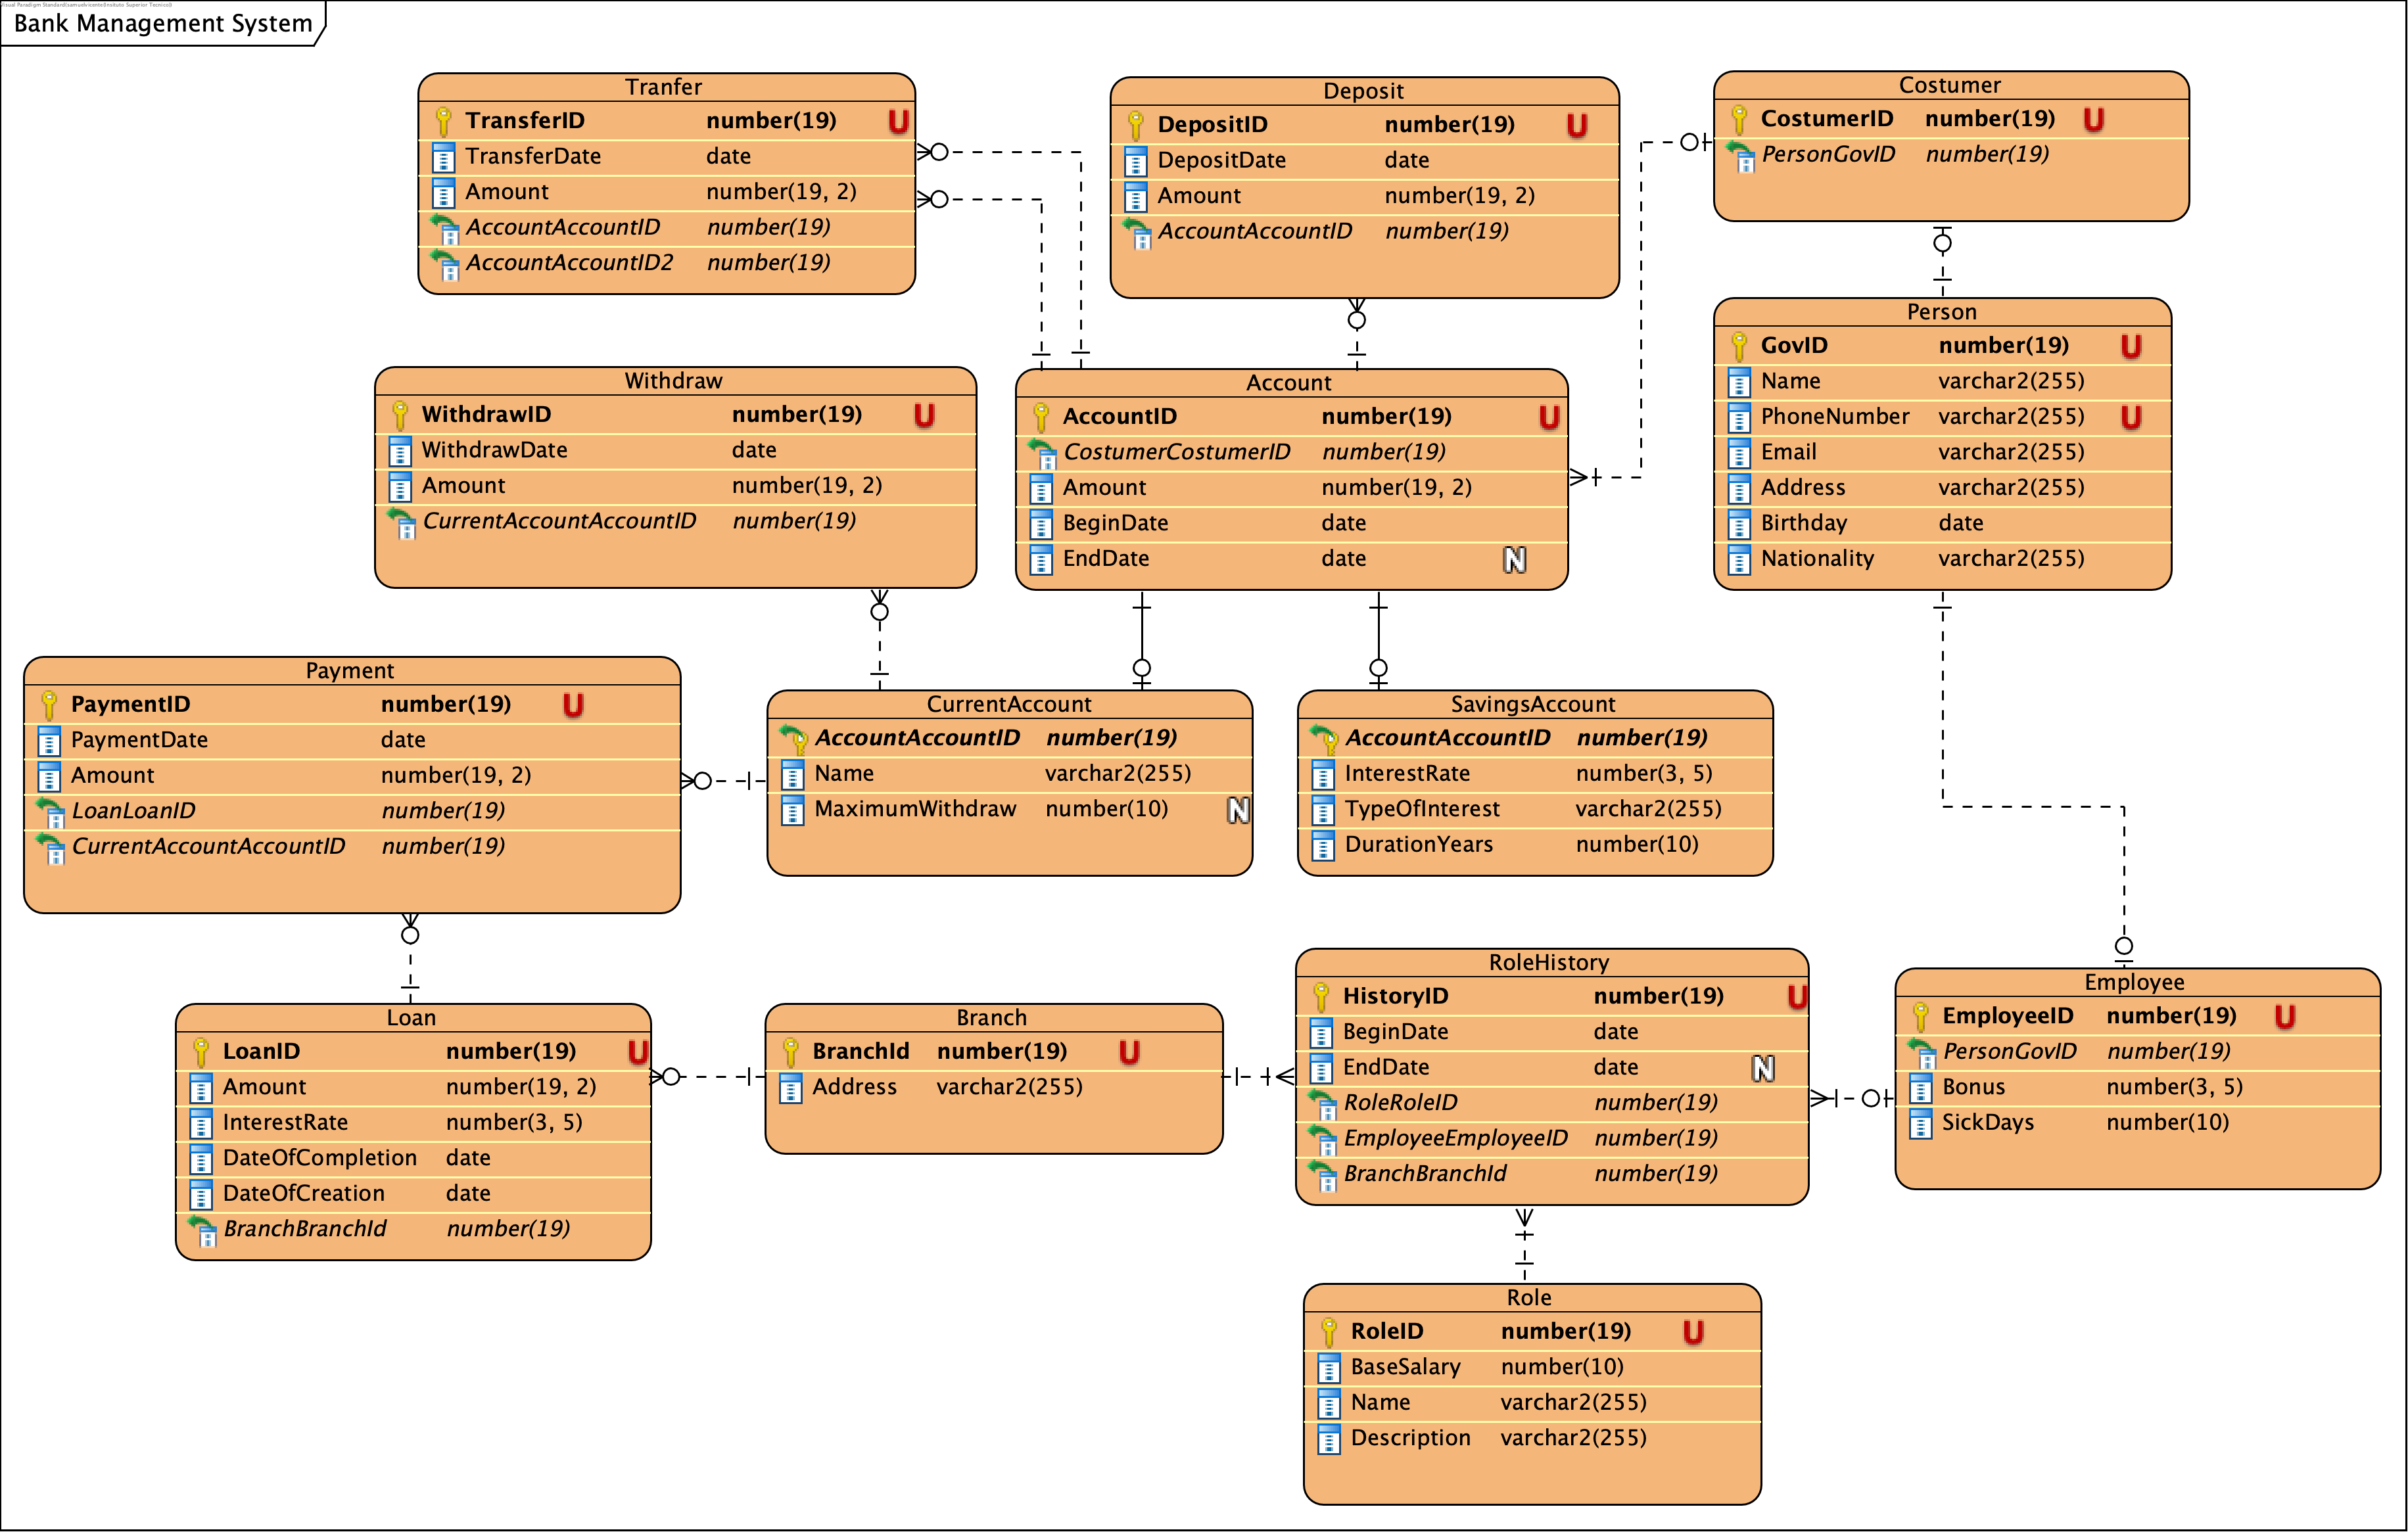
\includegraphics[width=\textwidth,height=\textheight,keepaspectratio]{bms}
\section{Schema}
\begin{lstlisting}[language=SQL]
CREATE TABLE Person (
  GovID       number(19) GENERATED AS IDENTITY, 
  Name        varchar2(255) NOT NULL, 
  PhoneNumber varchar2(255) NOT NULL UNIQUE, 
  Email       varchar2(255) NOT NULL, 
  Address     varchar2(255) NOT NULL, 
  Birthday    date NOT NULL, 
  Nationality varchar2(255) NOT NULL, 
  PRIMARY KEY (GovID));

CREATE TABLE Costumer (
  CostumerID  number(19) GENERATED AS IDENTITY, 
  PersonGovID number(19) NOT NULL, 
  PRIMARY KEY (CostumerID));

CREATE TABLE Employee (
  EmployeeID  number(19) GENERATED AS IDENTITY, 
  PersonGovID number(19) NOT NULL, 
  Bonus       number(3, 5) NOT NULL CHECK(Bonus>=0), 
  SickDays    number(10) NOT NULL CHECK(SickDays<10), 
  PRIMARY KEY (EmployeeID));

CREATE TABLE Account (
  AccountID          number(19) GENERATED AS IDENTITY, 
  CostumerCostumerID number(19) NOT NULL, 
  Amount             number(19, 2) NOT NULL CHECK(Amount>=0), 
  BeginDate          date NOT NULL, 
  EndDate            date, 
  PRIMARY KEY (AccountID));

CREATE TABLE Branch (
  BranchId number(19) GENERATED AS IDENTITY, 
  Address  varchar2(255) NOT NULL, 
  PRIMARY KEY (BranchId));

CREATE TABLE RoleHistory (
  HistoryID          number(19) GENERATED AS IDENTITY, 
  BeginDate          date NOT NULL, 
  EndDate            date, 
  RoleRoleID         number(19) NOT NULL, 
  EmployeeEmployeeID number(19) NOT NULL, 
  BranchBranchId     number(19) NOT NULL, 
  PRIMARY KEY (HistoryID));

CREATE TABLE Role (
  RoleID      number(19) GENERATED AS IDENTITY, 
  BaseSalary  number(10) NOT NULL CHECK(BaseSalary>0), 
  Name        varchar2(255) NOT NULL, 
  Description varchar2(255) NOT NULL, 
  PRIMARY KEY (RoleID));

CREATE TABLE Loan (
  LoanID           number(19) GENERATED AS IDENTITY, 
  Amount           number(19, 2) NOT NULL CHECK(Amount>0), 
  InterestRate     number(3, 5) NOT NULL, 
  DateOfCompletion date NOT NULL, 
  DateOfCreation   date NOT NULL, 
  BranchBranchId   number(19) NOT NULL, 
  PRIMARY KEY (LoanID));

CREATE TABLE Payment (
  PaymentID               number(19) GENERATED AS IDENTITY, 
  PaymentDate             date NOT NULL, 
  Amount                  number(19, 2) NOT NULL CHECK(Amount>0), 
  LoanLoanID              number(19) NOT NULL, 
  CurrentAccountAccountID number(19) NOT NULL, 
  PRIMARY KEY (PaymentID));

CREATE TABLE SavingsAccount (
  AccountAccountID number(19) NOT NULL, 
  InterestRate     number(3, 5) NOT NULL CHECK(InterestRate>0), 
  TypeOfInterest   varchar2(255) NOT NULL, 
  DurationYears    number(10) NOT NULL CHECK(DurationYears>0), 
  PRIMARY KEY (AccountAccountID));

CREATE TABLE Deposit (
  DepositID        number(19) GENERATED AS IDENTITY, 
  DepositDate      date NOT NULL, 
  Amount           number(19, 2) NOT NULL CHECK(Amount>0), 
  AccountAccountID number(19) NOT NULL, 
  PRIMARY KEY (DepositID));

CREATE TABLE Tranfer (
  TransferID        number(19) GENERATED AS IDENTITY, 
  TransferDate      date NOT NULL, 
  Amount            number(19, 2) NOT NULL CHECK(Amount>0), 
  AccountAccountID  number(19) NOT NULL, 
  AccountAccountID2 number(19) NOT NULL, 
  PRIMARY KEY (TransferID));

CREATE TABLE Withdraw (
  WithdrawID              number(19) GENERATED AS IDENTITY, 
  WithdrawDate            date NOT NULL, 
  Amount                  number(19, 2) NOT NULL CHECK(Amount>0), 
  CurrentAccountAccountID number(19) NOT NULL, 
  PRIMARY KEY (WithdrawID));

CREATE TABLE CurrentAccount (
  AccountAccountID number(19) NOT NULL, 
  Name             varchar2(255) NOT NULL, 
  MaximumWithdraw  number(10), 
  PRIMARY KEY (AccountAccountID));

ALTER TABLE Costumer ADD CONSTRAINT FKCostumer923053 FOREIGN KEY (PersonGovID) REFERENCES Person (GovID);

ALTER TABLE Employee ADD CONSTRAINT FKEmployee249023 FOREIGN KEY (PersonGovID) REFERENCES Person (GovID);

ALTER TABLE Account ADD CONSTRAINT FKAccount895601 FOREIGN KEY (CostumerCostumerID) REFERENCES Costumer (CostumerID);

ALTER TABLE RoleHistory ADD CONSTRAINT FKRoleHistor647811 FOREIGN KEY (RoleRoleID) REFERENCES Role (RoleID);

ALTER TABLE RoleHistory ADD CONSTRAINT FKRoleHistor516821 FOREIGN KEY (EmployeeEmployeeID) REFERENCES Employee (EmployeeID);

ALTER TABLE RoleHistory ADD CONSTRAINT FKRoleHistor171832 FOREIGN KEY (BranchBranchId) REFERENCES Branch (BranchId);

ALTER TABLE Loan ADD CONSTRAINT FKLoan357293 FOREIGN KEY (BranchBranchId) REFERENCES Branch (BranchId);

ALTER TABLE SavingsAccount ADD CONSTRAINT FKSavingsAcc25288 FOREIGN KEY (AccountAccountID) REFERENCES Account (AccountID);

ALTER TABLE Payment ADD CONSTRAINT FKPayment955503 FOREIGN KEY (LoanLoanID) REFERENCES Loan (LoanID);

ALTER TABLE Deposit ADD CONSTRAINT FKDeposit626030 FOREIGN KEY (AccountAccountID) REFERENCES Account (AccountID);

ALTER TABLE Tranfer ADD CONSTRAINT FKTranfer816388 FOREIGN KEY (AccountAccountID) REFERENCES Account (AccountID);

ALTER TABLE Tranfer ADD CONSTRAINT FKTranfer299653 FOREIGN KEY (AccountAccountID2) REFERENCES Account (AccountID);

ALTER TABLE Payment ADD CONSTRAINT FKPayment25568 FOREIGN KEY (CurrentAccountAccountID) REFERENCES CurrentAccount (AccountAccountID);

ALTER TABLE Withdraw ADD CONSTRAINT FKWithdraw546165 FOREIGN KEY (CurrentAccountAccountID) REFERENCES CurrentAccount (AccountAccountID);

ALTER TABLE CurrentAccount ADD CONSTRAINT FKCurrentAcc16041 FOREIGN KEY (AccountAccountID) REFERENCES Account (AccountID);
\end{lstlisting}

\section{Transactions}

\subsection{1:Changing Query}
\subsubsection{Description}
There is 5 CurrentAccount in the system. This transaction doubles the amount of the account that has the biggest value in the database.

\subsubsection{Input}
\subsubsection{Output}

\subsubsection{SQL}
\begin{lstlisting}[language=SQL]
BEGIN TRANSACTION
UPDATE Account 
SET amount = amount*2 
WHERE AccountID = (
    SELECT AccountID 
    FROM Costumer c 
    INNER JOIN Person p 
        ON p.GovID = c.PersonGovID 
    INNER JOIN Account 
        ON CostumerID = CostumerCostumerID 
    INNER JOIN CurrentAccount 
        ON AccountAccountID = AccountID 
    WHERE amount >= ALL(
        SELECT MAX(amount) 
        FROM Account 
    )
);
COMMIT
\end{lstlisting}

\subsection{2:Changing Query}
\subsubsection{Description}
This transaction preforms a withdraw of 100 units on the CurrentAccount with the AccountAccountID 1. To do this we must first check if the amount we want to withdraw is smaller than the CurrentAccount MaximumWithdraw, after that we update the amount and add an entry to the Withdraw ledger.

\subsubsection{Input}
\subsubsection{Output}

\subsubsection{SQL}
\begin{lstlisting}[language=SQL]
BEGIN TRANSACTION
UPDATE Account
SET amount =
    CASE 
        WHEN 100<(
            SELECT MaximumWithdraw 
            FROM CurrentAccount 
            WHERE AccountAccountID=1) 
          THEN amount - 100
        ELSE amount
    END
WHERE AccountID=(
    SELECT AccountAccountID 
    FROM CurrentAccount INNER JOIN Account 
        ON AccountID=AccountAccountID 
    WHERE AccountAccountID=1);

UPDATE Account
SET EndDate =
    CASE 
        WHEN amount=0 THEN CURRENT_DATE
        ELSE null
    END
WHERE AccountID = (
    SELECT AccountAccountID 
    FROM CurrentAccount INNER JOIN Account 
        ON AccountID=AccountAccountID 
    WHERE AccountAccountID=1);

INSERT INTO Withdraw(WithdrawDate, Amount, CurrentAccountAccountID) VALUES(CURRENT_DATE, 100, 1);
COMMIT
\end{lstlisting}

\end{document}
